%!Mode::"UTF-8"
\documentclass[12pt]{article}

% 页面设置
\usepackage{geometry}
\geometry{left=2.5cm, right=2.5cm, top=2.5cm, bottom=2.5cm}
\usepackage{graphicx}
\usepackage{ctex}
\usepackage{fontspec}
\usepackage{setspace}

% 代码设置
\usepackage{listings}
\usepackage{color}
\setmonofont{Consolas}
\definecolor{listing}{gray}{0.97}
\lstset{
	backgroundcolor=\color{listing},
	basicstyle=\footnotesize,
	numbers=left,
	numberstyle=\footnotesize,
	stepnumber=1,
	aboveskip={0.5\baselineskip},
	belowskip={0.5\baselineskip},
	columns=fullflexible,
	breaklines=true,
	breakatwhitespace=true,
	frame=single,
	basicstyle=\ttfamily,
	numberstyle=\ttfamily,
	tabsize=2
}

% 字体设置
\setmainfont{Times New Roman}
\setCJKmainfont{SimSun}
\setCJKsansfont{SimHei}

% 表格设置
\usepackage{makecell}
\newcommand{\addcell}[2][4]{\makecell{\zihao{#1}\textsf{#2}}}
\usepackage{titlesec}
\usepackage{booktabs}
\usepackage{tabularx}

% 设置图注、表注
\usepackage{caption}
\usepackage{bicaption}
\captionsetup{labelsep=quad, font={small, bf}, skip=2pt}
\DeclareCaptionOption{english}[]{
    \renewcommand\figurename{Fig.}
    \renewcommand\tablename{Table}
}
\captionsetup[bi-second]{english}

% 设置页眉
\usepackage{fancyhdr}
\pagestyle{fancy}
\fancypagestyle{preContent}{
    \fancyhead[L]{\zihao{-5} 物理化学实验}
    \fancyhead[C]{\zihao{-5} 实验七\ \ 氢氧化铁溶胶的制备及其性质研究}
    \fancyhead[R]{\zihao{-5} 1800011828\ 王宇哲}
}
\pagestyle{preContent}

%	设置首页页眉页脚
\fancypagestyle{plain}{
	\fancyhead[L]{\zihao{-5} 物理化学实验}
	\fancyhead[C]{\zihao{-5} 实验七\ \ 氢氧化铁溶胶的制备及其性质研究}
	\fancyhead[R]{\zihao{-5} 1800011828\ 王宇哲}
	\cfoot{}
}

% 设置标题格式
\titleformat*{\section}{\zihao{4}\sffamily}
\titleformat*{\subsection}{\zihao{-4}\sffamily}
\titleformat*{\subsubsection}{\zihao{-4}\sffamily}
\titlespacing*{\section}{0pt}{10pt}{10pt}
\titlespacing*{\subsection}{0pt}{10pt}{5pt}
\titlespacing*{\subsubsection}{0pt}{10pt}{5pt}

% 设置引用格式
\usepackage[super,round,comma,compress]{natbib}

\usepackage{amsmath}
\usepackage{amssymb}

%设置封面
\begin{document}
    % 标题页
    \begin{titlepage}
    	% 页眉
    	\thispagestyle{plain}
        % 图片
        \begin{figure}[h]
            \centering
            \includegraphics{pku.png}
        \end{figure}
        \vspace{24pt}
        % 标题
        \centerline{\zihao{-0} \textsf{物理化学实验报告}}
        \vspace{40pt} % 空行
        \begin{center}
            \begin{tabular}{cp{11.5 cm}}
                % 题目
                \addcell[2]{题目:\ } & \addcell[2]{氢氧化铁溶胶的制备及其性质研究} \\
                \cline{2-2}
            \end{tabular}
        \end{center}
        \vspace{20pt} % 空行
        \begin{center}
            \doublespacing
            \begin{tabular}{cp{5cm}}
                % 姓名
                \addcell{姓\phantom{空格}名:\ } & \addcell{王宇哲} \\
                \cline{2-2}
                % 学号
                \addcell{学\phantom{空格}号:\ } & \addcell{1800011828}\\
                \cline{2-2}
                % 组别
                \addcell{组\phantom{空格}别:\ } & \addcell{11组} \\
                \cline{2-2}
                % 实验日期
                \addcell{实验日期:\ } & \addcell{2020.11.25}\\
                \cline{2-2}
                % 室温
                \addcell{室\phantom{空格}温:\ } & \addcell{290.75\ K}\\
                \cline{2-2}
                % 大气压强
                \addcell{大气压强:\ } & \addcell{103.05\ kPa}\\
                \cline{2-2}
            \end{tabular}
            \begin{tabular*}{\textwidth}{c}
                \\ % 这是空行
                \\ % 这是空行
                \\ % 这是空行
                \\ % 这是空行
                \hline % 分割线
            \end{tabular*}
        \end{center}
        % 摘要
        \textsf{摘\ \ 要}\ \ 本实验使用凝结法制备了$\rm Fe(OH)_{3}$溶胶,利用热渗析法对其进行了初步纯化,使$\rm Fe(OH)_{3}$溶胶电导降为$396\  {\rm \mu S\cdot cm^{-1}}$。利用上一组同学制备的电导为$20.1\ \ {\rm \mu S\cdot cm^{-1}}$的$\rm Fe(OH)_{3}$溶胶进行聚沉实验,计算$\rm KCl$、$\rm K_{2}SO_{4}$、$\rm K_{3}Fe(CN)_{6}$溶液的聚沉值分别为$(4.3\pm 0.8)\ \ {\rm mmol\cdot dm^{-3}}$、$(0.06\pm 0.01)\ \ {\rm mmol\cdot dm^{-3}}$、$(0.019\pm 0.004)\ \ {\rm mmol\cdot dm^{-3}}$。通过溶胶电泳实验,计算溶胶电动电势$\zeta=(58\pm 3)\ \ {\rm mV}$。
        \\
        \\
        % 关键字
        \textsf{关键词}\ \ $\rm Fe(OH)_{3}$溶胶;胶体聚沉;溶胶电泳;电动电势
    \end{titlepage}

    \section{引言}
	略
               
\vbox{}        
    \section{实验部分}
    	\subsection{仪器和试剂}
    	$\rm FeCl_{3}$溶液$(10\%)$,$\rm AgNO_{3}$溶液$0.01\ \ {\rm mol\cdot dm^{-3}}$,$\rm KSCN$溶液$0.1\ \ {\rm mol\cdot dm^{-3}}$,$\rm KCl$溶液$0.04\ \ {\rm mol\cdot dm^{-3}}$,$\rm K_{2}SO_{4}$溶液$0.002\ \ {\rm mol\cdot dm^{-3}}$,$\rm K_{3}Fe(CN)_{6}$溶液$0.001\ \ {\rm mol\cdot dm^{-3}}$,$\rm 20000Da$透析袋;\par 
    	滴管,单口烧瓶,烧杯,试管,$\rm 5 mL$量筒,透析袋夹子;\par 
    	电加热套,电磁搅拌器,电导率仪,U型电泳管,稳压电泳仪,铂电极,水浴锅,秒表。
    
\vbox{}
    	 \subsection{实验内容\citealp{physchemlab}}
			\subsubsection{$\rm Fe(OH)_{3}$溶胶的制备}
在洁净的$\rm 250 \ \ mL$单口烧瓶中加入$\rm 100 \ \ mL$去离子水与搅拌磁子,加热至沸。一边搅拌一边缓慢滴加$\rm 5.0\ \ mL \ \ 10\% \ \ FeCl_{3}$溶液,加完后保持微沸状态继续搅拌加热$\rm 5\ \ min$,得到红棕色的氢氧化铁溶液。过程中不可补加水。
\subsubsection{$\rm Fe(OH)_{3}$溶胶的纯化}
将剪好的透析袋在去离子水中浸泡至变柔软,将透析袋一端用夹子夹好,装入去离子水试漏,浸泡在去离子水中备用。\par 
将制得的氢氧化铁溶胶倒入透析袋中,并将透析袋另一端用夹子夹好并测试是否有漏液。将密封好的透析袋置于装有已预热去离子水$\rm (60\sim 80\ \ ^{\circ }C)$的$\rm 1000\ \ mL$烧杯中,在电磁搅拌下进行透析。尽可能使透析袋转动起来以提高透析效率。\par 
在透析的前一个小时中,每隔$\rm 30\ \ min$更换一次水(水事先在水浴锅中预热备用)。第二次换水用$\rm KSCN$溶液检测透析液中的$\rm Fe^{3+}$离子,用$\rm AgNO_{3}$溶液检测$\rm Cl^{-}$离子,直至透析液中的$\rm Cl^{-}$离子浓度基本检测不出来为止,改为使用电导率仪测量透析液的电导率变化来监测透析速度,当电导率变化缓慢时可更换新的去离子水。直至透析液电导$<\rm 30 \ \ μS/cm$,再用
电导率仪测量溶胶的电导率。\par
将装有溶胶的透析袋置于盛有新换去离子水的烧杯中,并将写好溶胶电导值、姓名、学号信息的标签纸贴于该烧杯内壁。烧杯杯口用保鲜膜密封。放在指定位置储存,供下周实验的同学使用。 			
\subsubsection{溶胶聚沉实验}
用电导率仪测量上一组同学制备好的溶胶的电导,记录电导率值为$20.1\ \ {\rm \mu S/cm}$,符合实验要求。用量筒量取三份已经纯化好的溶胶各$5 \ \ {\rm mL}$装入三个试管中,分别滴加$0.04\ \ {\rm mol\cdot dm^{-3}}$的$\rm KCl$溶液,$0.002\ \ {\rm mol\cdot dm^{-3}}$的$\rm K_{2}SO_{4}$溶液,$0.001\ \ {\rm mol\cdot dm^{-3}}$的$\rm K_{3}Fe(CN)_{6}$溶液,不断摇动充分摇匀,用一个试管盛放$\rm 5 \ \ mL$原溶胶做参比,记录开始出现明显聚沉现象所滴溶液的滴数。
			\subsubsection{溶胶电泳实验}
配制电导值与溶胶电导值相同的$\rm KCl$溶液作为辅助液,用电导率仪测量辅助液电导率值为$20.1\ \ {\rm \mu S/cm}$。\par 
彻底清洗电泳管至内壁不挂水珠,用去离子水洗3次,再用少量溶胶润洗2次;将电泳管固定在支架上,从中间管加溶胶至刻度$\rm 4\ \ cm$附近;用滴管交替向左右两管沿管壁小心滴加辅助液,直至液面达刻度$\rm 8\sim 9\ \ cm$。开始加辅助液时较慢,使液滴沿管壁流下,防止液面振荡。当发生液面振荡界面模糊,应立即停下来,等稳定后再加。当液面高度离界面较高时,可适当加快滴加速度。\par 
将电极插入电泳仪的“+”、“-”插孔中,打开电泳仪预热。将两电极插入装有辅助液的烧杯中,调节两极间电压稳定在$\rm 100\pm 5\ \ V$。断开回路,小心地将电极插入电泳管中大约液面下$1\ \ \rm cm$,正极插入左管,负极插入右管,记录电极位置和界面位置。连通电路开始电泳实验并计时。观察溶胶与辅助液的界面位置,每隔$\rm 1\ \ min$记录正极和负极的界面位置,测6组以上数据,同时观察并记录界面状态以及电极表面的变化。\par 
测完后关闭电源,用棉线沿电泳管的中心线测量两电极间距离,测量三次取平均值,计算电动电势。
\vbox{}
 \section{数据与结果}
 \subsection{实验数据记录及处理}
 \subsubsection{$\rm Fe(OH)_{3}$溶胶的纯化}
 记录$\rm Fe(OH)_{3}$溶胶纯化过程中更换水的次数、时间间隔及离子检测结果,检测不出$\rm Cl^{-}$后用电导率仪测量并记录每次换水时透析液及最后溶胶的电导率,结果如\textbf{表1}所示,其中“$+$”表示离子检出,“$-$”表示粒子未检出。
 \begin{table}[h]
 	\centering
 	\zihao{5}
 	\bicaption{$\rm Fe(OH)_{3}$溶胶的纯化过程}{Purification process of $\rm Fe(OH)_{3}$ sol}
 	\begin{tabular}{cccccc}
 		\toprule
 		编号 & 透析时长$t/{\rm min}$ & ${\rm Cl^{-}}$检测 & ${\rm Fe^{3+}}$检测 & 透析液电导/${\rm \mu S\cdot cm^{-1}}$ & 胶体电导/${\rm \mu S\cdot cm^{-1}}$  \\
 		\midrule
 		1 & 38.2 & $+$ & $+$ &  & \\
 		2 & 31.0 & $+$ & $+$ &  &\\
 		3 & 20.4 & $+$ & $-$ &  &\\
 		4 & 29.4 & $-$ & $-$ & 346 &\\
 		5 & 16.4 &  &  & 82.9 &\\
 		6 & 31.3 &  &  & 100.8 &\\
 		7 & 21.0 &  &  & 29.2 & 396\\
 		\bottomrule
 	\end{tabular}
 \end{table}
 \par

 
\subsubsection{溶胶聚沉实验与聚沉值的计算}
向$\rm Fe(OH)_{3}$溶胶中分别滴加$c=0.04\ \ {\rm mol\cdot dm^{-3}}$的$\rm KCl$溶液、$c=0.002\ \ {\rm mol\cdot dm^{-3}}$的$\rm K_{2}SO_{4}$溶液、$c=0.001\ \ {\rm mol\cdot dm^{-3}}$的$\rm K_{3}Fe(CN)_{6}$溶液,记录胶体发生聚沉时所加入的电解质溶液的滴数$n$,按$0.05\ \ {\rm mL/}$滴计算加入电解质溶液的体积$V$,结果如\textbf{表2}所示。
\begin{table}[h]
	\centering
	\zihao{5}
	\bicaption{$\rm Fe(OH)_{3}$溶胶聚沉实验数据}{$\rm Fe(OH)_{3}$ sol coagulation experiment data}
	\begin{tabular}{ccccc}
		\toprule
		编号 & 溶液种类 & $c/{\rm mol\cdot dm^{-3}}$ & $n$ & $V/{\rm mL}$  \\
		\midrule
		1 & $\rm KCl$ & $\rm 0.040$ & $12$ & $0.6$  \\
		2 & $\rm K_{2}SO_{4}$ & $\rm 0.0020$ & $3$ & $0.15$  \\
		3 & $\rm K_{3}Fe(CN)_{6}$ & $\rm 0.0010$ & $2$ & $0.1$ \\
		\bottomrule
	\end{tabular}
\end{table}
\par
聚沉值$a$是一定条件下刚刚足以引起某种溶胶聚沉的电解质浓度,单位一般为$\rm mmol\cdot dm^{-3}$。试管中$\rm Fe(OH)_{3}$胶体溶液的体积$V_{0}={\rm 5.0\ \ mL}$,加入电解质溶液的体积为$V$,浓度为$c$,则聚沉值的计算公式为
$$
a=\frac{cV}{V+V_{0}}
$$
认为$V_{0}$的不确定度$\sigma_{V_{0}}=0.1\ \ {\rm mL}$,每一滴电解质溶液体积的不确定度$\sigma_{V_{n}}=0.01\ \ {\rm mL}$,加入电解质溶液的滴数为$n$,则加入电解质溶液体积的不确定度为
$$
\sigma_{V}=n\sigma_{V_{n}}=0.01n
$$
故计算聚沉值$a$的不确定度
$$
\sigma_{a}=\frac{cV_{0}V}{(V_{0}+V)^{2}}\sqrt{\dfrac{\sigma_{V_{0}}^{2}}{V_{0}^{2}}+\frac{\sigma_{V}^{2}}{V^{2}}}
$$
\par
以$\rm KCl$溶液为例,计算聚沉值
$$
a=\frac{0.040\ \ {\rm mol\cdot dm^{-3}}\times 0.6\ \ {\rm mL}}{0.6\ \ {\rm mL}+5.0\ \ {\rm mL}}=4.3\ \ {\rm mmol \cdot dm^{-3}}
$$
聚沉值的不确定度
$$
\sigma_{a}=\frac{0.040\ \ {\rm mol\cdot dm^{-3}}\times 5.0\ \ {\rm mL}\times 0.6\ \ {\rm mL}}{(0.6 \ \ {\rm mL}+5.0\ \ {\rm mL})^{2}}\sqrt{\frac{0.1^{2}}{5.0^{2}}+\frac{0.12^{2}}{0.6^{2}}}=0.8\ \ {\rm mmol\cdot dm^{-3}}
$$
故$\rm KCl$的聚沉值
$$
a=(4.3\pm 0.8)\ \ {\rm mmol\cdot dm^{-3}}
$$
依此计算三种溶液的聚沉值,结果如\textbf{表3}所示。
\begin{table}[h]
	\centering
	\zihao{5}
	\bicaption{不同电解质聚沉值的计算结果}{Calculation results of different electrolyte coagulation values}
	\begin{tabular}{cccc}
		\toprule
		编号 & 溶液种类 & $c/{\rm mol\cdot dm^{-3}}$ & $a/{\rm mmol\cdot dm^{-3}}$  \\
		\midrule
		1 & $\rm KCl$ & $\rm 0.040$ & $4.3\pm 0.8$  \\
		2 & $\rm K_{2}SO_{4}$ & $\rm 0.0020$ & $0.06\pm 0.01$  \\
		3 & $\rm K_{3}Fe(CN)_{6}$ & $\rm 0.0010$ & $0.019\pm 0.004$ \\
		\bottomrule
	\end{tabular}
\end{table}
\par
$\rm KCl$、$\rm K_{2}SO_{4}$、$\rm K_{3}Fe(CN)_{6}$分别为1-1、2-1、3-1型电解质,负离子分别带1、2、3个负电荷。在聚沉实验中,带正电的$\rm Fe(OH)_{3}$胶体在电解质溶液中负离子的作用下发生聚沉,从\textbf{表3}可以看出,负离子所带电荷越高,聚沉值$a$越小,说明该电解质溶液使$\rm Fe(OH)_{3}$胶体聚沉的能力越强。
\subsubsection{溶胶电泳实验与两电极间距离的测量}
在$\rm Fe(OH)_{3}$溶胶电泳实验过程中,记录正负两极的界面位置随时间的变化,结果如\textbf{表4}所示,其中$t$为电泳实验进行的时间,$h_{L}$为左侧界面位置,$h_{R}$为右侧界面位置。
\begin{table}[h]
	\centering
	\zihao{5}
	\bicaption{$\rm Fe(OH)_{3}$溶胶电泳实验数据}{$\rm Fe(OH)_{3}$ sol electrophoresis experimental data}
	\begin{tabular}{cccc}
		\toprule
		编号 & $t/{\rm s}$ & $h_{L}/{\rm cm}$ & $h_{R}/{\rm cm}$  \\
		\midrule
		1 & $0$ & $3.84$ & $3.55$  \\
		2 & $65$ & $3.76$ & $3.68$  \\
		3 & $129$ & $3.62$ & $3.75$  \\
		4 & $188$ & $3.57$ & $3.82$  \\
		5 & $247$ & $3.45$ & $3.90$  \\
		6 & $309$ & $3.36$ & $4.01$  \\
	    7 & $370$ & $3.27$ & $4.18$  \\
	    8 & $430$ & $3.15$ & $4.26$  \\
	    9 & $489$ & $3.08$ & $4.39$  \\
	   10 & $550$ & $2.94$ & $4.50$  \\
		\bottomrule
	\end{tabular}
\end{table}
\par
在$\rm Fe(OH)_{3}$溶胶电泳实验进行过程中,观察界面状态以及电极表面的变化。随着电泳实验的进行,左侧界面在下降过程中越来越模糊,而右侧界面在上升过程中越来越清晰;两侧电极表面有少量气泡产生,右侧比左侧产生的气泡更多。\par 
测量完成后关闭电源,用棉线沿电泳管的中心线测量两电极间的距离$l$,重复测量三次,结果如\textbf{表5}所示。
\begin{table}[h]
	\centering
	\zihao{5}
	\bicaption{两电极间距离测量数据}{Measurement data of distance between two electrodes}
	\begin{tabular}{cccc}
		\toprule
		编号 & 1 & 2 & 3  \\
		\midrule
		 $l/{\rm cm}$& $22.65$ & $23.30$ & $23.25$  \\
		\bottomrule
	\end{tabular}
\end{table}
\par
计算两电极间距离$l$的平均值
$$
l=\frac{22.65+23.30+23.25}{3}\ \ {\rm cm}=23.07\ \ {\rm cm}
$$ 
两电极间距离$l$的不确定度
$$
\sigma_{l}=\sqrt{\frac{(22.65-23.07)^{2}+(23.30-23.07)^{2}+(23.25-23.07)^{2}}{3-1}}\ \ {\rm cm}=0.4\ \ {\rm cm}
$$
故
$$
l=(23.1\pm 0.4)\ \ {\rm cm}
$$
\vbox{}
 \subsection{数据处理结果与分析}
 \subsubsection{胶体界面时间-迁移距离关系图与平均泳动速度计算}
$\rm Fe(OH)_{3}$胶体左侧界面迁移距离
$$s_{L}=h_{L_{0}}-h_{L}
$$
右侧界面迁移距离
$$s_{R}=h_{R}-h_{R_{0}}
$$
根据以上公式及\textbf{表4}数据,计算左右两侧胶体界面的迁移距离随时间$t$的变化,结果如\textbf{表6}所示。
\begin{table}[h]
	\centering
	\zihao{5}
	\bicaption{$\rm Fe(OH)_{3}$溶胶电泳界面迁移距离的计算结果}{Calculation result of migration distance of $\rm Fe(OH)_{3}$ sol electrophoresis interface}
	\begin{tabular}{cccc}
		\toprule
		编号 & $t/{\rm s}$ & $s_{L}/{\rm cm}$ & $s_{R}/{\rm cm}$  \\
		\midrule
		1 & $0$ & $0$ & $0$  \\
		2 & $65$ & $0.08$ & $0.13$  \\
		3 & $129$ & $0.22$ & $0.20$  \\
		4 & $188$ & $0.27$ & $0.27$  \\
		5 & $247$ & $0.39$ & $0.35$  \\
		6 & $309$ & $0.48$ & $0.46$  \\
		7 & $370$ & $0.57$ & $0.63$  \\
		8 & $430$ & $0.69$ & $0.71$  \\
		9 & $489$ & $0.76$ & $0.84$  \\
		10 & $550$ & $0.90$ & $0.95$  \\
		\bottomrule
	\end{tabular}
\end{table}
\par
根据\textbf{表5}数据作出$s_{R}-t$、$s_{L}-t$关系的散点图,并用python SciPy lingress进行线性拟合,作出拟合直线,如\textbf{图1}所示。
\begin{figure}[h]
	\centering
	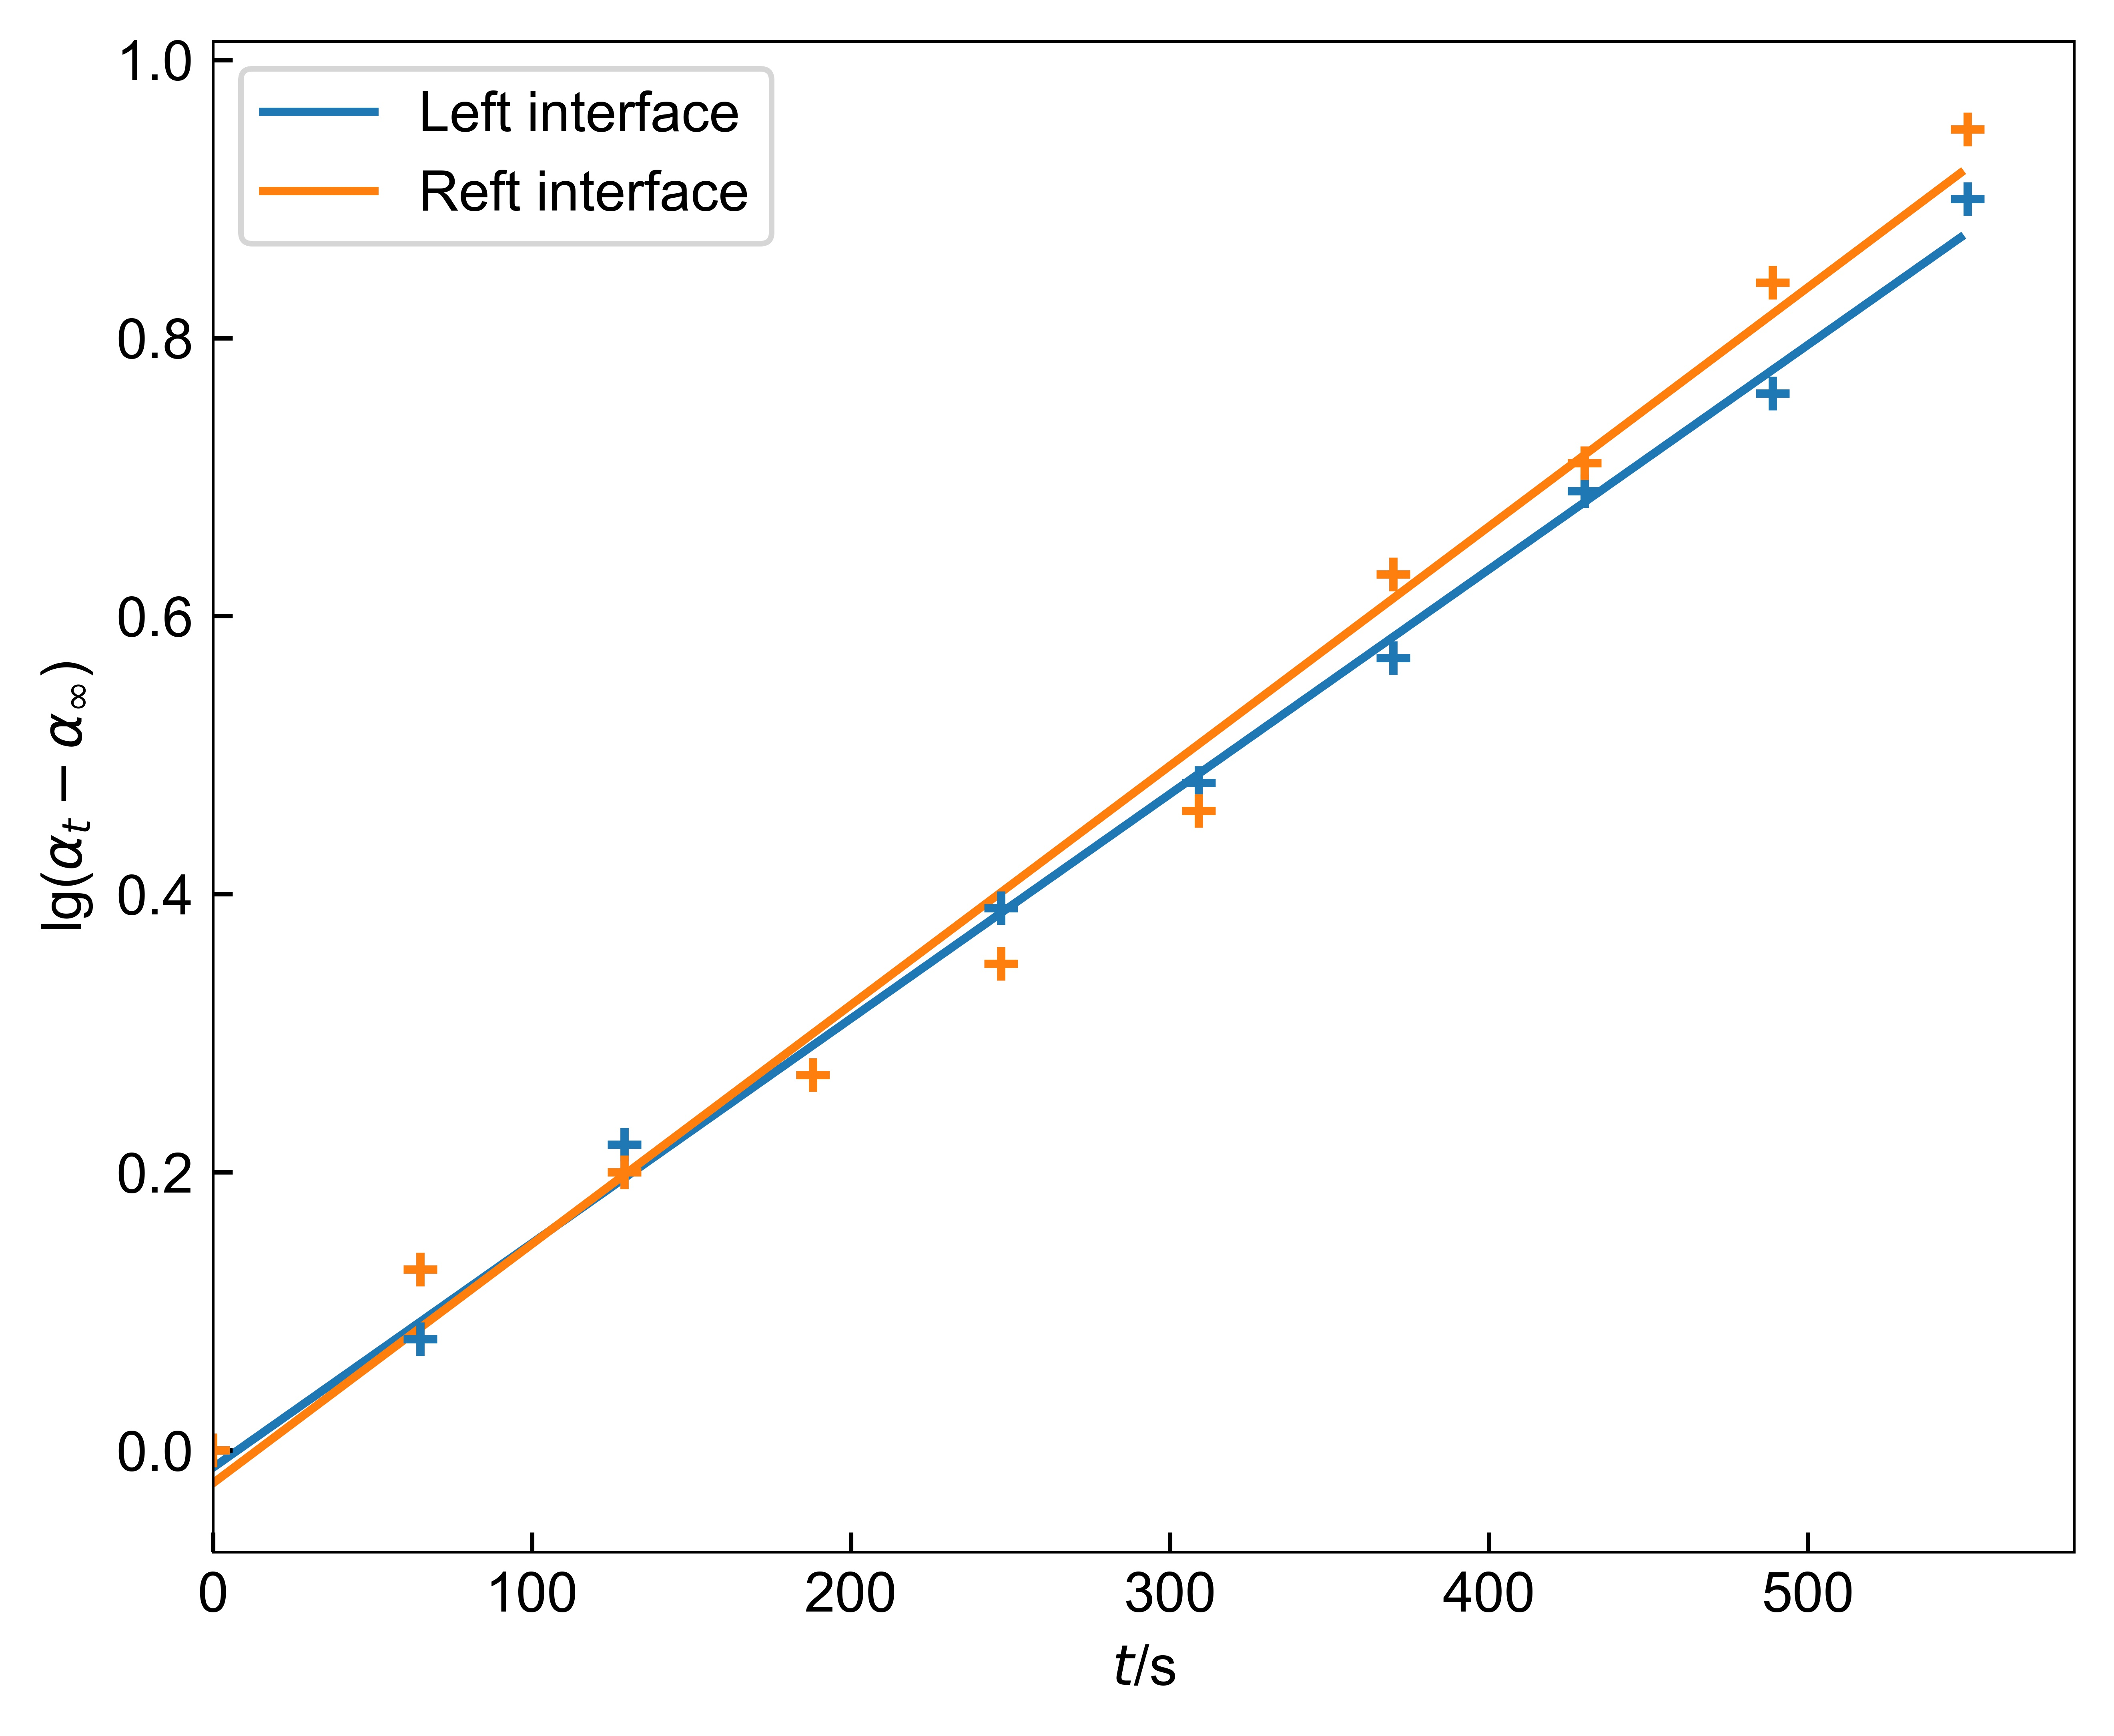
\includegraphics[width=0.65\textwidth]{1.jpg}
	\bicaption{$\rm Fe(OH)_{3}$溶胶电泳时间$t$-界面迁移距离$s$关系图}{$s-t$ Diagram of $\rm Fe(OH)_{3}$ sol electrophoresis interface}
\end{figure}
\par
拟合直线的方程为
$$
s_{L}/{\rm cm}=(0.00161\pm 0.00003)t/{\rm s}-(0.01\pm 0.01),\   \  R=0.9984
$$
$$
s_{R}/{\rm cm}=(0.00172\pm 0.00006)t/{\rm s}-(0.02\pm 0.02),\   \  R=0.9947
$$
拟合直线的斜率即为两侧界面迁移的平均速度,即
$$
v_{L}=(0.00161\pm 0.00003)\ \ {\rm cm\cdot s^{-1}}
$$
$$
v_{R}=(0.00172\pm 0.00006)\ \ {\rm cm\cdot s^{-1}}
$$
计算两侧界面迁移的平均速度
$$
v=\dfrac{v_{L}+v_{R}}{2}=0.00166\ \ {\rm cm\cdot s^{-1}}
$$
界面迁移速度的不确定度
$$
\sigma_{v}=\sqrt{\sigma_{v_{R}}^{2}+\sigma_{v_{L}}^{2}}=0.00007\ \ {\rm cm\cdot s^{-1}}
$$
即平均泳动速度为
$$
v=(0.00166\pm 0.00007)\ \ {\rm cm\cdot s^{-1}}
$$
\subsubsection{电动电势的计算}
利用公式
$$
\zeta=\frac{\eta s l}{\varphi t \varepsilon_{r} \varepsilon_{0}}=\frac{\eta v l}{\varphi  \varepsilon_{r} \varepsilon_{0}}
$$
计算$\rm Fe(OH)_{3}$胶体的电动电势,其中两电极间距离$l=(23.1\pm 0.4){\rm cm}$,平均泳动速度(界面迁移平均速度)$v=(0.00166\pm 0.00007)\ \ {\rm cm\cdot s^{-1}}$,两电极间电势差$\varphi=100\ \ {\rm V}$。查阅\textit{CRC Handbook of Chemistry and Physics}\citealp{crc},得到真空介电常数$\varepsilon_{0}=8.8542\times 10^{-12}\ \ {\rm F\cdot m^{-1}}$,$20\ \ {\rm ^{\circ}C}$时水的相对介电常数$\varepsilon_{r}=80.10$;查阅《物理化学实验(第四版)》书后附录表D.4-15\citealp{textbook},知$t=17\ \ {\rm ^{\circ}C}$时,水的黏度$\eta=1.083\ \ {\rm mPa\cdot s}$,$t=18\ \ {\rm ^{\circ}C}$时,水的黏度$\eta=1.056\ \ {\rm mPa\cdot s}$,实验室实际温度$t=17.6\ \ {\rm ^{\circ}C}$,近似认为$17\ \ {\rm ^{\circ}C\sim 18\ \ ^{\circ}C}$范围内水的黏度与温度呈线性关系,计算$t=17.6\ \ {\rm ^ {\circ}C}$时水的黏度
$$
\eta=1.083+\frac{1.083-1.056}{17-18}\times 0.6\ \ {\rm mPa\cdot s}=1.067\ \ {\rm mPa\cdot s}
$$
\par 
代入各项数据,得
$$
\zeta=\frac{\eta v l}{\varphi  \varepsilon_{r} \varepsilon_{0}}=\frac{1.067\ \ {\rm mPa\cdot s} \times 1.66\times 10^{-3}\ \ {\rm cm\cdot s} \times 23.1\ \ {\rm cm}}{100\ \ {\rm V}  \times 80.10 \times 8.8542\times 10^{-12}\ \ {\rm F\cdot m^{-1}}}=58\ \ {\rm mV}
$$
不确定度

$$
\sigma_{\zeta}=\zeta\sqrt{\frac{\sigma_{l}^{2}}{l^{2}}+\frac{\sigma_{v}^{2}}{v^{2}}}=58 \times \sqrt{\frac{0.4^{2}}{23.1^{2}}+\frac{0.00007^{2}}{0.00166^{2}}} \ \ {\rm mV}=3\ \ {\rm mV}
$$

故$\rm Fe(OH)_{3}$溶胶的电动电势
$$
\zeta=(58\pm 3) \ \ {\rm mV}
$$
\vbox{}
 	 \section{讨论与结论}
		\subsection{实验讨论}
 			\subsubsection{计算电动电势$\zeta$的误差分析}
在计算电动电势的过程中,$\sigma_{l}$和$\sigma_{v}$都对电动电势的不确定度$\sigma_{\zeta}$造成了贡献。其中,电极间距$l$的贡献为
$$
\frac{\sigma_{l}^{2}}{l^{2}} / \frac{\sigma_{\zeta}^{2}}{\zeta^{2}}=14.4\%
$$
电泳速度$v$的贡献为
$$
\frac{\sigma_{v}^{2}}{v^{2}} / \frac{\sigma_{\zeta}^{2}}{\zeta^{2}}=85.6\%
$$
可见电动电势的不确定度主要是由电泳速度$v$的不确定度造成的。在计算电泳速度时,通过对电泳时间$t$-界面迁移距离$s$进行直线拟合,根据斜率得到电泳速度$v$,在此过程中,可能的误差来源有:
\par (1)电泳过程中界面迁移并非匀速,是由静止状态逐渐开始迁移的,拟合得到的界面迁移速度与稳恒状态时的界面迁移速度有所不同,造成误差;\par 
(2)在电泳过程中,胶体与辅助液的分界面不够清晰(尤其是左管,因为左管的界面随电泳进行而变模糊),导致读数时难以分辨界面位置,造成误差;\par 
(3)实验过程中读取界面迁移距离$s$和从计时器读取时间$t$不完全同步,两者有时间上的先后,且每次测量时情况不同,导致$s-t$图直线的位置发生偏移,误差变大。\par 
需要说明的是,在计算电动电势时,$\eta$、$\varphi$等物理量也具有一定的误差,例如由于未准确测定胶体的温度,仅以室温作为胶体温度,使水的黏度$\eta$的实际值与代入值不完全一致;并且作为$\rm Fe(OH)_{3}$胶体的黏度与纯水有一定的不同,但在实验过程中认为该不同可以忽略,未测量胶体的黏度,引入了一定的误差。但这些误差与界面迁移速度$v$的不确定度相比是较小的,为减小$\zeta$测定的不确定度,关键是更准确地测量$v$。
 	 	\subsubsection{实验改进}
根据上述分析,在实际实验中,为了减小电动电势$\zeta$测量的不确定度,可以采取以下措施:\par 
(1)尽可能缓慢小心滴加辅助液,保持胶体与辅助液界面清晰,再开始电泳实验;
\par 
(2)用手机等将整个电泳过程录像,事后仔细估读胶体界面的位置,通过这种方法也能够避免读取界面位置与读取时间的不同步。


 	 \subsection{实验结论}
本实验使用凝结法制备了$\rm Fe(OH)_{3}$溶胶,利用热渗析法对其进行了初步纯化,使$\rm Fe(OH)_{3}$溶胶电导降为$396\  {\rm \mu S\cdot cm^{-1}}$。利用上一组同学制备的电导为$20.1\ \ {\rm \mu S\cdot cm^{-1}}$的$\rm Fe(OH)_{3}$溶胶进行聚沉实验,计算$\rm KCl$、$\rm K_{2}SO_{4}$、$\rm K_{3}Fe(CN)_{6}$溶液的聚沉值分别为$(4.3\pm 0.8)\ \ {\rm mmol\cdot dm^{-3}}$、$(0.06\pm 0.01)\ \ {\rm mmol\cdot dm^{-3}}$、$(0.019\pm 0.004)\ \ {\rm mmol\cdot dm^{-3}}$。通过溶胶电泳实验,计算溶胶电动电势$\zeta=(58\pm 3)\ \ {\rm mV}$。


 

   

\vbox{}

\bibliographystyle{achemso}
\bibliography{a}



\end{document}